\documentclass{article}
\usepackage[utf8]{inputenc}
\usepackage{blindtext}
\usepackage{quotchap}
\usepackage{graphicx}
\setlength{\parindent}{12pt}
\setlength{\parindent}{0cm}
\usepackage[catalan]{babel}
\usepackage{lmodern}
\newtheorem{theorem}{Teorema}
\usepackage{amsfonts}

%Definició de la ela geminada per tal que accepti el punt volat del teclat
\def·#1{%
  \ifmmode
    \cdot #1
    %\csname normal@char\string"\endcsname l%
  \else%
    \def\argument{#1}%
    \if\argument l%
      \leftllkern=0pt\rightllkern=0pt\raiselldim=0pt%
      \setbox0\hbox{l}\setbox1\hbox{l\/}\setbox2\hbox{.}%
      \advance\raiselldim by \the\fontdimen5\the\font
      \advance\raiselldim by -\ht2%
      \leftllkern=-.25\wd0%
      \advance\leftllkern by \wd1%
      \advance\leftllkern by -\wd0%
      \rightllkern=-.25\wd0%
      \advance\rightllkern by -\wd1%
      \advance\rightllkern by \wd0%
      \allowhyphens\discretionary{-}{l}%
      {\hbox{}\kern\leftllkern\raise\raiselldim\hbox{.}%
        \kern\rightllkern\hbox{l}}\allowhyphens%
    \else
      \if\argument L%
        \leftllkern=0pt\rightllkern=0pt\raiselldim=0pt%
        \setbox0\hbox{L}\setbox1\hbox{L\/}\setbox2\hbox{.}%
        \advance\raiselldim by .5\ht0%
        \advance\raiselldim by -.5\ht2%
        \leftllkern=-.125\wd0%
        \advance\leftllkern by \wd1%
        \advance\leftllkern by -\wd0%
        \rightllkern=-\wd0%
        \divide\rightllkern by 6%
        \advance\rightllkern by -\wd1%
        \advance\rightllkern by \wd0%
        \allowhyphens\discretionary{-}{L}%
        {\hbox{}\kern\leftllkern\raise\raiselldim\hbox{.}%
           \kern\rightllkern\hbox{L}}\allowhyphens%
      \else
        #1
      \fi
    \fi
  \fi
  }

\title{Xarxes neuronals amb la llibreria Torch per predir ingresos a la UCI de l'hospital  Clinic}
\author{Jaume Betriu i Tort}
\date{Setembre 2021}

\begin{document}

\maketitle
\section{Intel·ligència artificial, \textit{machine learning} i \textit{deep learning}}
Abans de parlar de \textit{deep learning}, neurones, xarxes neuronals, funcions d'activació... (nocions que més endavant estudiarem en profunditat) cal parlar del conjunt que engloba tots aquests conceptes: La intel·ligència artificial. 

\vspace{5mm}

Una manera ràpida i concisa per definir el que és la intel·ligència artificial (IA) és el següent enunciat:

\begin{quote}

\textit{La intel·ligència artificial es l'esforç d'automatitzar tasques intel·lectuals normalment portades a terme per humans}
\qauthor{François Chollet, \textit{Deep Learning with Python}}
\end{quote}
Com ja hem comentat la IA és un conjunt que conté els subconjunts \textit{machine learning} i \textit{deep learning} i aquests dos estan relacionats entre ells tal i com mostra la següent figura:

\\
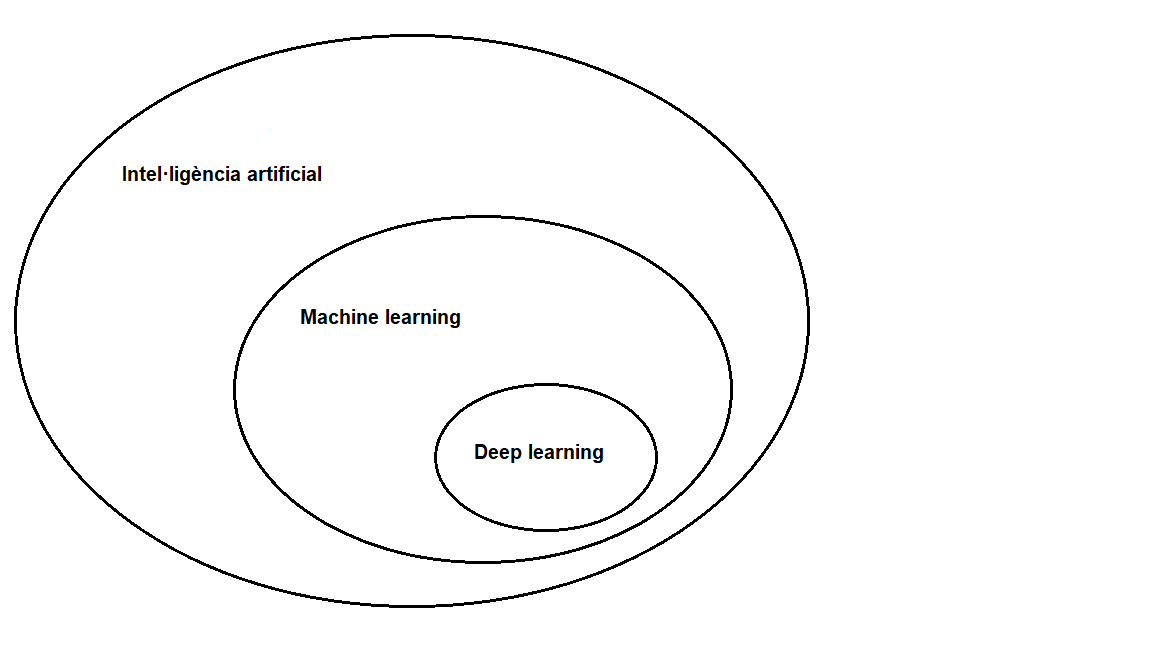
\includegraphics[scale=0.45]{relacio IA.png}
\\
 
Per tant, com podem apreciar en la figura, no tots els procediments inclosos en el camp de la IA inclouen algun tipus d'aprenentatge. Per posar un exemple els primers programes que jugaven a escacs estaven dissenyats a partir de regles implementades per programadors i durant un període considerable de temps es va creure que es podria assolir la fita d'una IA amb capacitat de raonament quasi humana mitjançant un conjunt suficientment gran de regles explicites dissenyades pels desenvolupadors. Aquest enfoc s'anomena IA simbòlica i va dominar el camp de la intel·ligència artificial des de la dècada dels 50 fins als 80.

Lamentablement ,tot i que les IA simbòliques van donar resultats prou satisfactoris en problemes com jugar a escacs, poc a poc aquest enfoc va quedar obsolet al ser intractables per resoldre problemes com la classificació d'imatges, el reconeixement de veu i la traducció entre d'altres. Va ser doncs quan un nou enfoc va començar a agafar força: El \textit{machine learning}, o per la seva traducció: Aprenentatge Automàtic (AA).

\subsection{Machine learning o Aprenentatge Automàtic}

Pot una màquina anar més enllà del que ha estat explícitament programada per portar a terme? Podria un algoritme aprendre automàticament a base d'alimentar-lo amb dades? Un ordinador ens pot arribar a sorprendre?

Aquestes preguntes ens introdueixen a un nou camp dins la IA, l'Aprenentatge Automàtic. Com ja hem comentat, en els programes de IA simbòlics els programadors introdueixen una sèrie de regles i dades que seran processades utilitzant aquestes regles per extreure respostes. En canvi en Aprenentatge Automàtic el programador introdueix les dades i també les respostes lligades a aquestes dades per tal que l'algoritme ens doni com a resultat les regles. Aquestes regles més endavant les podem aplicar a noves dades per tal d'obtenir noves respostes. La següent figura explica esquemàticament aquest fet:

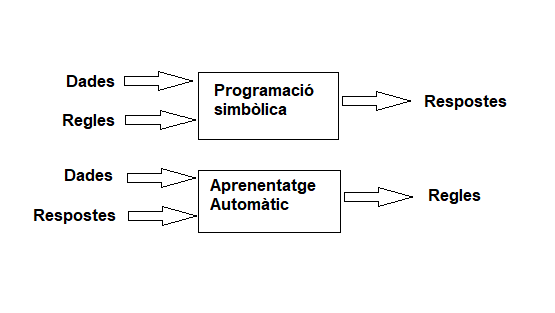
\includegraphics[scale=1]{Esquema AA.png}

Podríem dir que els sistemes AA son entrenats més que no pas programats explícitament. La idea principal es que se li presenten al sistema una sèrie d'exemples associats amb una resposta i l'algoritme troba una estructura estadística que permetrà al sistema deduir aquestes regles per fer prediccions amb noves dades.

Per exemple podríem entrenar un model d'AA amb un conjunt de fotografies de gats i gossos etiquetades a mà per un humà. Una vegada entrenat el model podríem comprovar com de bo és utilitzant un conjunt d'imatges de test (que no s'han fet servir per entrenar el model) i verificant que la etiqueta que els hi associa el model siguin les correctes. Dependrà de diversos factors que aquest model sigui bo o no per la tasca per la qual l'hem entrenat com ara que el conjunt d'exemples per l'entrenament sigui suficientment gran, que l'estructura estadística del model sigui adequada per la labor en qüestió, que no l'haguem sobre-ajustat a les dades d'entrenament...

Resumint: per crear un model i fer Aprenentatge Automàtic necessitem en essència dos ingredients:

\begin{itemize}
    \item Dades d'entrada per entrenar el model. En el cas que hem presentat abans aquestes dades serien les fotografies dels gats i els gossos prèviament etiquetades de forma manual.
    \item Una manera de mesurar si l'algoritme esta fent una bona feina a l'hora de classificar. Aquesta mesura s'utilitzarà per ajustar el model per tal de que doni millors resultats com veurem més endavant.
\end{itemize}

Per tant, podríem dir que la paraula Aprenentatge (\textit{learning}) en aquest context descriu una mena de procés automàtic per trobar una representació millor de les dades.

\subsection{Introducció al deep learning}

Com ja hem comentat el deep learning (aprenentatge profund) és un subconjunt del machine learning. Un enfoc que posa èmfasi en nivells o capes d'aprenentatge ordenades successivament. La paraula deep (profund) no es refereix a que els models de deep learning gaudeixin d'un enteniment més profund de les qüestions, simplement fa referència a la idea d'ordenar diverses capes d'aprenentatge una rere l'altre per construir els models. La quantitat de capes que contribueixen en la construcció del model s'anomena la profunditat del model. 

Considerem un primer exemple per posar una mica de llum a la qüestió: Suposem que volem dissenyar un algoritme que donada una imatge d'un nombre escrit a mà per una persona sigui capaç de saber quin és el nombre en qüestió. Un esquema de com un model de deep learning funcionaria és el següent:

\\
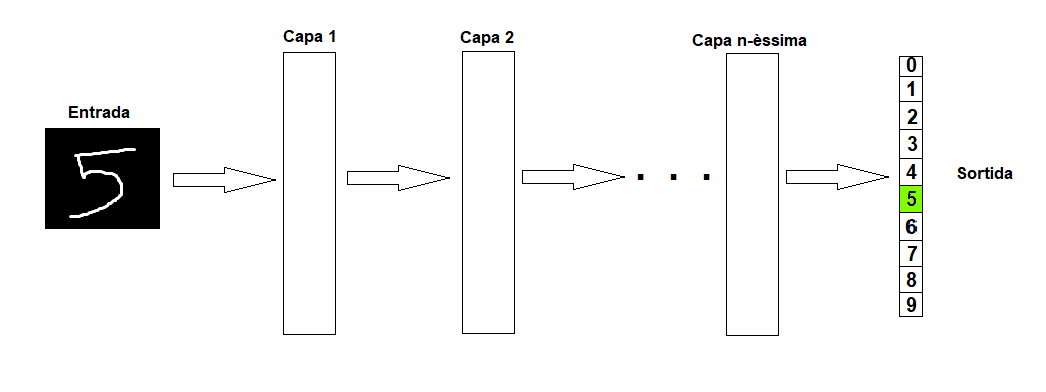
\includegraphics[scale=0.55]{esquema deep.png}
\\

Cada capa fa una sèrie de transformacions a certs paràmetres de les dades d'entrada i passa la informació a las següent capa. Podem pensar que aquesta informació va passant per diferents filtres i es va polint per tal de que la informació de sortida sigui útil per, en el cas que estem considerant, classificar el nombre. Evidentment aquestes transformacions no son aleatòries i, de fet, que el  model sigui prou bo per la tasca que li hem encomanat dependrà de com es fan. La idea doncs es que aquestes transformacions es facin d'acord als exemples d'entrenament que li hem donat al model. Quin tipus de transformacions es fan exactament i com es passa la informació de capa en capa ho estudiarem en profunditat en les següents seccions. 

En aquest projecte ens fixarem en les representacions en nivells anomenades xarxes neuronals, que son pràcticament el paradigma dominant en deep learning.

\section{Xarxes neuronals}

Una xarxa neuronal és, tal i com suggereix el seu nom, una serie de neurones interconnectades entre si i ordenades per nivells o capes. El primer nivell s'anomena nivell d'entrada (\textit{input layer} en anglès), l'últim nivell es coneix com nivell de sortida (\textit{output layer}) i ens referirem als nivells intermedis com nivells ocults (\textit{hidden layers}). En el cas de que entre dues capes successives (capa $n$ i capa $n+1$) totes les neurones de la cap $n$ estiguin connectades a totes les neurones de la capa $n+1$ direm que la xarxa és una xarxa neuronal totalment connectada. 

Però que és una neurona? Té alguna cosa a veure amb les neurones que tots coneixem? \\

Podríem dir que la resposta és que sí. D'ara endavant coneixerem com a neurona a un node que pren un valor (un \textit{input}) d'entrada, fa certes computacions per transformar aquesta entrada i expulsa un valor de sortida en dos passos:

\begin{itemize}
    \item Combinació de l'input o entrada
    \item Funció d'activació
\end{itemize}
seguint el següent esquema:

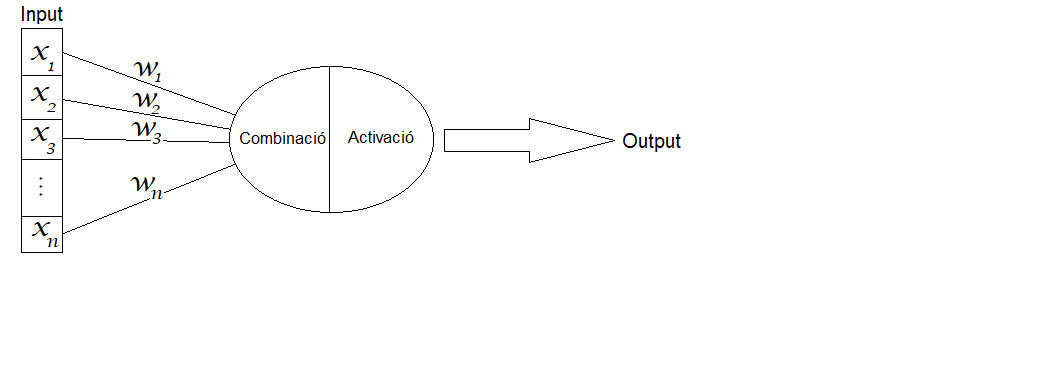
\includegraphics[scale=0.8]{esquema neurona.png}

Com podem veure el funcionament és molt senzill. Introduïm a la neurona una sèrie de dades en forma de input multiplicades per uns certs pesos ($w_1, \cdots,w_n$), combinem aquests valors i a continuació fem una transformació anomenada activació.

Anem per parts, com es fa aquesta combinació? Tenim diverses possibilitats que presentarem però la que més es fa servir és la primera:

\begin{itemize}
    \item Suma ponderada: $$z(x_1,\cdots,x_n)=\sum ^n_{i=1} w_i x_i$$
    \item Màxim o mínim: $$z(x_1,\cdots,x_n)=max(w_1 x_1,w_2 x_2,\cdots ,w_n x_n)$$
                         $$z(x_1,\cdots,x_n)=min(w_1 x_1,w_2 x_2,\cdots ,w_n x_n)$$
    \item Lògic AND($\wedge$)/OR($\vee$): (en cas de que l'input siguin valors binaris) $$z(x_1,\cdots,x_n)=w_1 x_1 \wedge w_2 x_2 \wedge \cdots \wedge w_n x_n$$
    $$z(x_1,\cdots,x_n)=w_1 x_1 \vee w_2 x_2 \vee \cdots \vee w_n x_n$$
\end{itemize}
Com ja hem comentat la més comú és la suma ponderada i és la que utilitzarem d'ara endavant per defecte en excepció dels casos que especifiquem que farem servir un altre tipus de combinació.

És comú afegir al pas de combinació un element $b$ que anomenem biaix que és suma al resultat. Per exemple, en el cas de la suma ponderada l'afegiríem de la següent manera:

$$z(x_1,\cdots,x_n)=\sum ^n_{i=1} w_i x_i +b$$ 


\subsection{Funcions d'activació}
Parlem ara de l'activació. L'activació no és més que aplicar al valor que extraiem de la combinació una funció preestablerta. Existeixen un gran ventall de funcions d'activació i en aquest projecte utilitzarem les següents:

\begin{itemize}

    
\item \textbf{Funció sigmoide}:
    $$\sigma(x)=\frac{1}{1+e^{-x}}$$
    
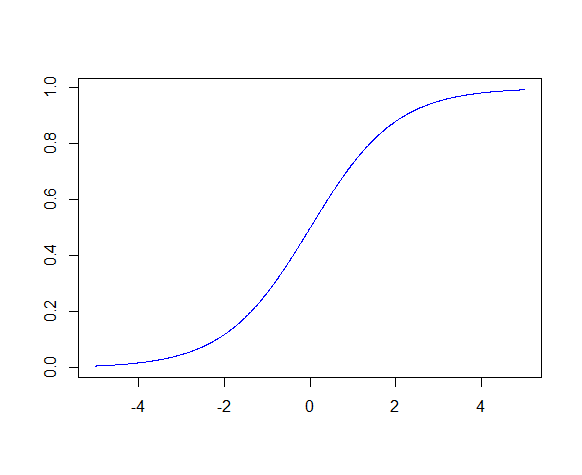
\includegraphics[scale=0.7]{Sigmoid gràfic.png}

La mateixa funció que s'utilitza amb la regressió logística. Útil en el cas de que ens interessi un output entre 0 i 1, per exemple en el cas de que el output desitjat sigui una probabilitat. A diferència de la funció de pas, la sigmoide sí que és diferenciable.

    
\item \textbf{Funció ReLU:}
    $$f(x)=max(0,x)$$

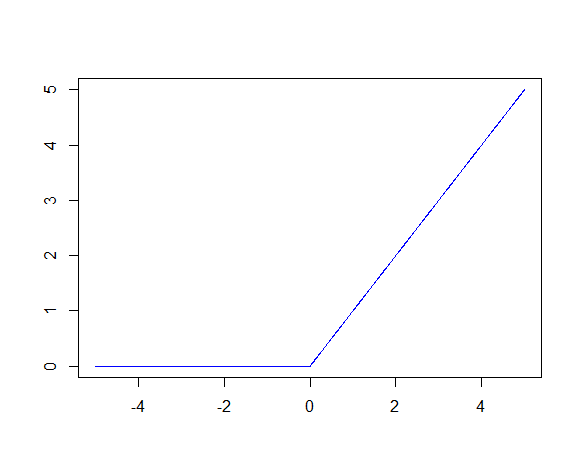
\includegraphics[scale=0.7]{relu.png}

Simple i sorprenentment molt útil a la pràctica ja que el seu gradient es molt fàcil de calcular.

\item \textbf{Funció softmax}

La funció softmax és un cas especial de funció d'activació que combina l'output de diverses neurones de la mateixa capa.

Si posem $z_j$ com el resultat de el pas de combinació de la neurona $j$ i considerem $z=(z_1, \cdots, z_K )$ on $K$ és la dimensió de la capa definim la funció softmax com:

$$S(z)_j = \frac{e^{z_j}}{\sum ^K _{i=1} e^{z_i}} $$

Si ens fixem en la funció softmax ens adonarem que si fem la suma de tots els ouptuts obtenim:

$$\sum _{i=1} ^{K} S(z)_i = 1$$ 

És lògic doncs pensar en els ouputs com la distribució de probabilitat entre $K$ possibles categories, molt útil en problemes de classificació com per exemple el cas ja mencionat del nombres escrits a mà. 

\end{itemize}

\section{D'un grapat d'operacions a un model d'intel·liència artificial}

Arribats a aquest punt ja sabem tots els elements que constitueixen una xarxa neuronal i les operacions que transformen els inputs en ouputs a mida que avancen per les diferents capes. La pregunta doncs és com ens pot ajudar aquesta estructura a resoldre problemes? Quines condicions s'han de complir per tal que una xarxa neuronal pugui arribar a ser útil per tal d'afrontar reptes com el reconeixement d'imatges? 

En aquesta secció parlarem del número de neurones, de capes, funcions de cost i com optimitzar-les i de com podem utilitzar aquests conceptes a l'hora de dissenyar models predictius útils i funcionals. Començarem parlant de les dimensions de les xarxes.

\subsection{Profunditat, complexitat i estructura de les xarxes neuronals}

Seleccionar un nombre òptim de capes i un nombre òptim de neurones per cada una de les capes pot ser una labor força complicada. Per norma general afegir neurones a una capa concreta o afegir noves capes a una xarxa millorarà la capacitat predictiva del model, però cal matisar molt aquesta afirmació. És cert que una xarxa neuronal profunda (amb més capes) serà capaç de comprendre estructures molt més complexes i afegint neurones permetrem al model crear noves característiques basades en l'output de les capes anteriors.

\ 

No hi han normes generals de com s'ha de definir l'estructura d'una xarxa neuronal però depenent de quin sigui el nostre objectiu les podem classificar en dos grans grups:

\begin{itemize}
    \item \textbf{Arquitectura per regressió: } En cas de que el nostre objectiu sigui resoldre un problema de regressió ens decantarem per estructures on l'última capa de la xarxa consisteixi en una sola neurona, com per exemple:
    
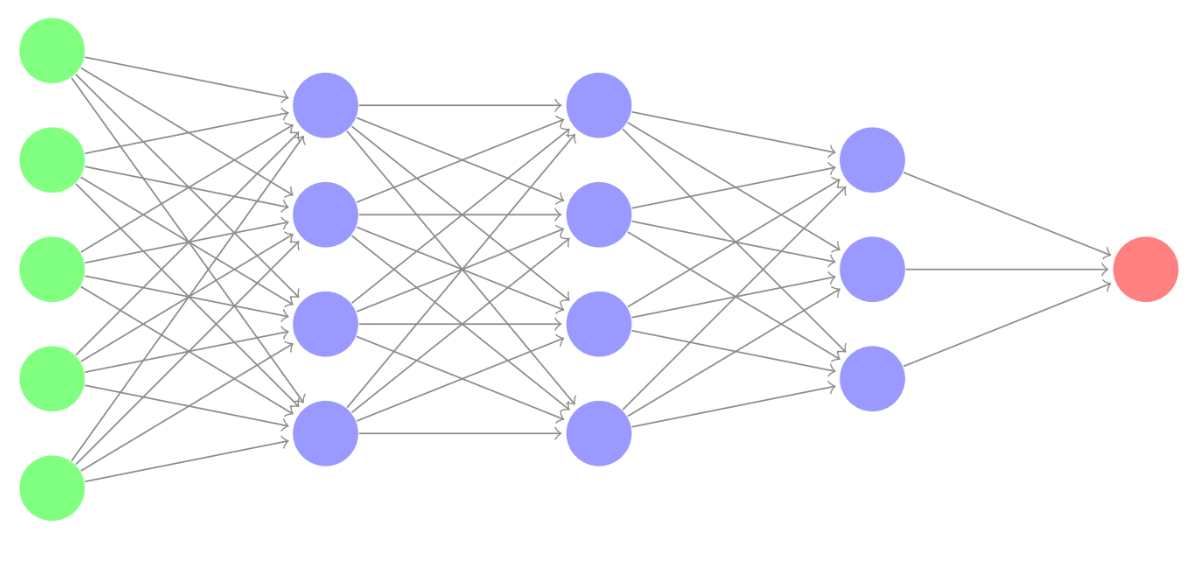
\includegraphics[scale=0.26]{regression_structure.png}
    
    \item \textbf{Arquitectura per classificació: } Quan ens enfrontem a problemes de classificació és essencial que la última capa de la nostra xarxa tingui el mateix nombre de neurones com classes tenim per classificar. A més a més, com ja hem comentat, és molt útil utilitzar l'activació softmax en aquesta última capa en aquest cas. Un exemple seria:
    
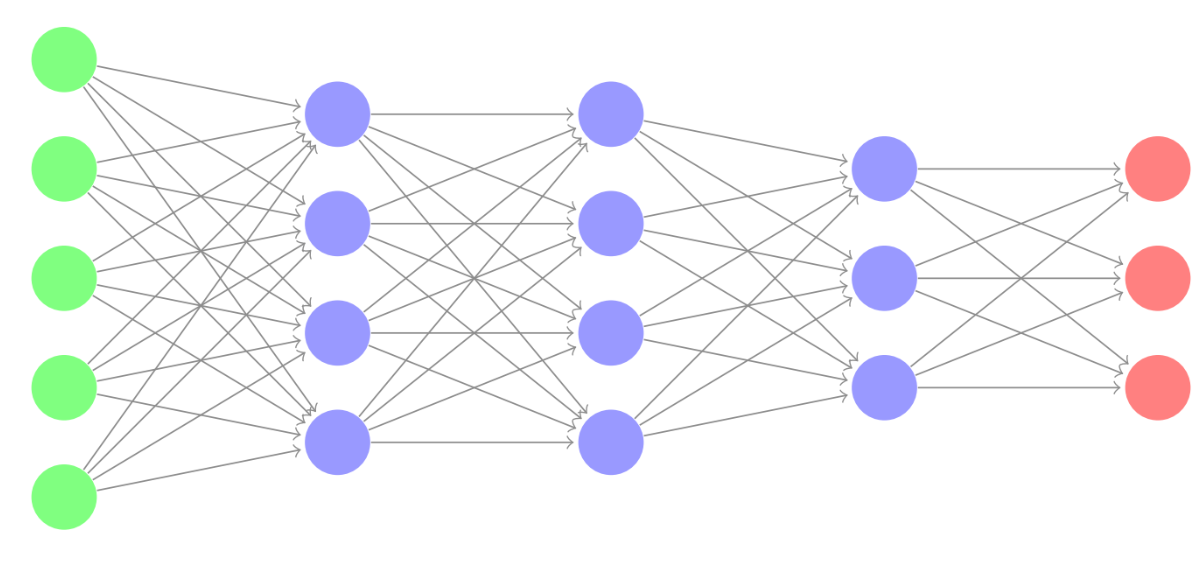
\includegraphics[scale=0.26]{classification_structure.png}


\end{itemize}


Tot i aixo hem de tenir especial cura a l'hora de definir les dimensions de la nostra xarxa per tal d'evitar l'enemic numero 1 dels models de AA: el sobreajustament. Parlarem en profunditat d'aquesta qüestió més endavant ja que és un dels problemes més recurrents a l'hora de crear models de deep learning.

\subsection{Funcions de cost, optimització i entrenament}

Com ja hem vist, cada neurona esta constituïda per una combinació de l'input d'entrada al qual se li aplica tot seguit una funció d'activació. Aquesta primera combinació conté uns elements que hem anomenat pesos i el biaix:

$$(w_1, \cdots,w_n,b)$$

que també reben el nom de paràmetres entrenables. Aquests elements contindran la informació que la xarxa ha anat aprenent al exposar-la a les dades d'entrenament. Per tal d'entrenar el model i adaptar-lo a les dades d'entrenament el primer pas es definir una manera de mesurar si el nostre algoritme és bo o no a l'hora de modelar aquestes. Llavors, d'alguna manera, el nostre objectiu serà aconseguir reduir al màxim aquests errors amb l'esperança que aixo ens permeti fer prediccions encertades amb noves dades. 

Per tal de desenvolupar més en profunditat aquest pas, cal que parlem d'un concepte fonamental. Les funcions de cost.

\subsubsection{Funcions de cost}

Les funcions de cost són funcions que ens ajudaran a mesurar com de bé (o com de malament) el nostre model fa prediccions dins les nostres dades d'entrenament. Podem trobar-ne de molts tipus diferents i depenent de si el nostre és un problema de regressió o de classificació haurem d'inclinar-nos per un tipus o un altre. Tot i així, totes comparteixen la mateixa estructura:

\ 

Suposem que hem creat un model $f$ que depèn d'uns paràmetres $w$ modificables. Suposem també que tenim un input $x$ el qual ens agradaria que el nostre model transformés en un output $y$. Llavors és raonable pensar en una manera de mesurar com de lluny està la predicció que fa el model $f$ amb l'input $x$ i el valor real $y$. És a dir, la funció de cost té la forma general:

$$L(w) = distància(f_w(x),y)$$

En el cas concret de les xarxes neuronals els paràmetres $w$ són els pesos i el biaix. Fixem-nos que com més petit sigui el valor de la funció, més aprop estaran les prediccions dels valors reals i més precís serà el nostre model. Vegem algunes funcions de cost típiques:

\begin{itemize}
    \item \textbf{Error quadràtic mitjà}
    
Si posem com $(y_1, \cdots, y_N)$ els valors reals a predir i $(\hat{y_1}, \cdots, \hat{y_N})$ les prediccions que ens retorna la xarxa definim l'error quadràtic mitjà com:

$$L_{MSE} = \frac{1}{N} \sum ^N _{i=1} (y_i - \hat{y_i})^2 $$

Molt utilitzada en problemes de regressió.

\item \textbf{Entropia creuada categòrica}

L'entropia creuada categòrica o funció de cost logarítmica s'utilitza en problemes de classificació. Considerem una xarxa amb $K$ neurones a la última capa i l'output té l'activació softmax.

\ 

Suposem també que volem fer $N$ prediccions per classificar $N$ instàncies entre $M$ categories. Suposem que per portar a terme tal labor dissenyem una xarxa neuronal amb $M$ neurones a la última capa i activació softmax. Per tant, per cada instància $i$ el model ens tornara $M$ probabilitats $\hat{p_{ij}}$ on aquesta és la probabilitat d'assignar la categoria $j$ a la instància $i$. Llavors definim la funció de cost logarítmica com:

$$L_{log} = -\frac{1}{N} \sum ^N _{i=1} \sum ^M _{j=1} y_{ij} log(\hat{p_{ij}}) $$

On $y_{ij}$ és un indicador binari que és $1$ si la categoria $j$ és la correcta per la instància $i$ i $0$ en cas contrari. Notem que només els termes de la categoria correcta per cada una de les instàncies contribueixen a la suma i observem que un classificador perfecte tindria $L_{log} = 0$ i valors progressivament més grans indicarien classificadors menys exactes.
\end{itemize}

\subsubsection{Entrenament del model}

Com ja hem anat introduint, la manera d'entrenar una xarxa consistirà en modificar d'una manera concreta els pesos i biaixos del model per tal que modeli correctament les dades d'entrenament. Per tant, el procés d'entrenament consistirà en utilitzar un mètode iteratiu per anar refinant aquests paràmetres i a cada pas utilitzar la nostra funció de cost de preferència per testejar si hi ha hagut millora. És a dir, aquest pas consisteix en optimitzar la funció de cost respecte als paràmetres $w$ i $b$.  

Pensem un moment en la funció de cost $L$. Si analitzem les seves components ens adonarem que, com ja hem fet notar al definir-la, si tenim un número fixat $N$ de instàncies en les nostres dades d'entrenament $L$ només depèn dels paràmetres $w, b$. És lògic doncs utilitzar el gradient de la funció $L$ per tal de trobar un mínim d'aquesta.

\ 

És conegut que el sentit oposat a on apunta el gradient d'una funció en un punt indica la direcció i el sentit de màxim decreixement.  Per tant, la nostra estratègia podria ser utilitzar un algoritme iteratiu com el següent:

$$x_{t+1} = x_t - \eta \nabla_{x} L(x_t) $$

On $\nabla_{x} L(x_t)$ és el vector gradient de $L$ en el punt $x_t$ i $\eta$ és un paràmetre d'aprenentatge. 

\ 

Aquest algoritme no ens assegura trobar el mínim global en casos no convexos però pot ser molt útil per trobar mínims locals i amb cada iteració tenim l'esperança que el punt $x_t$ convergeixi cap a un d'aquests mínims. Posats en aquesta situació només ens cal aclarir un fet, com calculem el gradient $ \nabla_{x} L$?

\subsubsection{Backpropagation}

Tornant al exemple de la xarxa que hem posat per exemple al parlar de l'estructura de regressió si calculem el nombre de paràmetres entrenables (incloent els biaixos) obtenim:

$$6·4 + 5·4 + 5·3 +4 = 63$$

És a dir, cal optimitzar $L$ en funció de $63$ paràmetres que a més a més han sofert composició de les funcions d'activació. Una labor pràcticament impossible i no escalable d'enfocar de la manera tradicional (calculant l'expressió de $L$ i derivant parcialment respecte els seus paràmetres). Cal buscar un nou enfoc més eficient i el mètode de la Backpropagation (propagació enrere) és una bona solució. Abans de presentar-la, ens caldrà introduir una mica de notació i enunciar un teorema ja conegut per tots, la regla de la cadena:

\begin{theorem}[Regla de la cadena:] \\

Siguin $f$, $g$ funcions continues sobre els reals d'una variable. Llavors la derivada de la composició $g(f(x))$ respecte $x$ satisfà:
$$\frac{\partial (g \circ f)}{\partial x} = \frac{\partial g}{\partial f} \cdot \frac{\partial f}{\partial x} $$
\end{theorem}

\textbf{Notació matemàtica:}

\begin{itemize}
    \item $n_l =$ Nombre de neurones a la capa $l$. Suposarem doncs que $n_0$ serà la dimensió de la primera capa i del input.
    
    \item $X \in M_{n_o \times m}(\mathbb{R})$ és la matriu que conté totes les instàncies. En un context de programació, es el nostre dataframe.
    
    \item $W^{[l]} \in M_{n_l \times n_{l-1}} (\mathbb{R})$ denota la matriu que conté els pesos que connecten la capa $l-1$ amb la capa $l$. \\
    Particularment l'element de la fila $j$, columna $k$ denotat per $w_{jk} ^{l}$ és el pes de la connexió entre la neurona j de la capa $l$ i la neurona $k$ de la capa $l-1$.
    
    \item $b^{[l]}$ és un vector de  mida $n_l$ que denota el biaix de la capa $l$. Els elements $b_j ^{[l]}$ denoten el biaix de la neurona $j$ en la capa $l$.
    
    \item $z^{[l]}$ és un vector de mida $n_l$ que conté la combinació de la capa $l-1$.
    
    \item $g$ la funció d'activació com ara la funció ReLU o sigmoide. \\
    Llavors si $S \in M_{c \times d} (\mathbb{R})$ denotarem per $g(M) \in M_{c \times d} (\mathbb{R})$ la matriu obtinguda al aplicar la funció $g$ component a component. El cas particular $d=1$ és la notació per vectors.
    
    \item Denotem $a^{[l]} \in M_{n_l \times 1} (\mathbb{R})$ l'output de la capa $l$. En particular en una xarxa amb $L$ capes denotem per $a^{[L]}$ l'output de la xarxa neuronal i per conveni $a^{[0]}$ el vector de inputs.
    
\end{itemize}

Llavors tindrem:

$$z_j^{[l]}= \sum _{k=1}^{n_{l-1}} w_{jk}^{[l]} \cdot a_k^{[l-1]} + b_j^{[l]} $$
$$a_j^{[l]} = g(z_j^{[l]}) $$

o en forma matricial:

$$z^{[l]} = W^{[l]} \cdot  a^{[l-1]}+b^{[l]}$$
$$a^{[l]} = g(z^{[l]})$$

Aplicant de manera recursiva l'expressió anterior capa a capa obtindrem l'output de la xarxa $a^{[L]}$ i definirem l'error del model amb la funció $L(y,a^{[L]})$ on $y$ és la categoria correcte de l'exemple en el que estem treballant. 

\ 

Al cap i a la fi, com l'element $a^{[L]}$ depèn dels paràmetres $W^{[l]}$ i $b^{[l]}$. Per tant la funció de cost $L$ també dependrà d'aquests paràmetres. Per tant, modificant-los obtindrem resultats de $L$ diferents. El nostre objectiu doncs és el de minimitzar $L$ modificant aquests paràmetres utilitzant, com ja hem comentat, la regla de la cadena i el gradient utilitzant el mètode de la Backpropagation (propagació cap enrere). Aquest algorisme consistirà en aplicar la regla de la cadena recursivament per anar calculant les derivades parcials de $L$ respecte tots els paràmetres. Posem un exemple:

\ 

Suposem que la nostra xarxa és un classificador binari. És a dir, el valor real esperat és o bé $1$ o bé $0$. Llavors si prenem com a funció de cost la logarítmica tindrem:

$$L(y, a^{[L]}) = -[y \cdot log(a^{[L]}) + (1-y) \cdot log(1-a^{[L]})] \Rightarrow \frac{\partial L}{\partial a^{[L]}} = - \left( \frac{y}{a^{[L]}} - \frac{1-y}{1-a^{[L]}}) \right) $$

Per tan, si volem calcular la derivada parcial de $L$ respecte $w^{[l]}_{jk}$ considerem els altres paràmetres com a constants i apliquem la regla de la cadena:

$$ \frac{\partial L}{\partial w^{[l]}_{jk}} = \frac{\partial L}{\partial a^{[l]}_j} \cdot \frac{\partial a_j ^{[l]}}{\partial z^{[l]}_j} \cdot \frac{\partial z_j ^{[l]}}{\partial w^{[l]}_{jk}}$$

Notem que per fer aquests càlculs cal saber els valors de $z^{[l]}$ i $a^{[l]} \ \forall l=1,\ldots,L$ que s'han calculat en el procés de calcular $a^[L ]$. Una vegada calculat el gradient podem recórrer a diferents mètodes iteratius per tal d'obtenir valors que minimitzin la funció de cost.

\subsubsection{Algoritmes d'optimització}

Ja hem comentat que una possible estratègia és utilitzar l'algoritme iteratiu:

$$x_{t+1} = x_t - \eta \nabla_{x} L(x_t) $$

amb l'esperança de que els punts $x_t$ convergeixin cap a un mínim global o local. Utilitzant aquest algoritme a cada pas calcularem el gradient de $L$ utilitzant el total de totes les dades disponibles. Aquest fet converteix en intractable aquest enfoc en la majoria de casos en els que desitgem entrenar el nostre model amb grans datasets. Cal buscar altres variants més ràpides i eficients:

\begin{itemize}
    \item \textbf{Descens estocàstic del gradient}
    
    En aquest cas en comptes d'utilitzar el total de totes les nostres dades per calcular el gradient, utilitzarem una sola observació $v^i$ amb la seva respectiva classificació $u^i$ per calcular una aproximació del gradient:
    
    $$ x_{t+1} = x_t - \eta \nabla_{x} L(x_t /  v^i:u^i) $$
    
    Evidentment aquest mètode és molt més ràpid ja que només tenim en compte una sola observació, però per altra banda pot ser molt inestable i no convergir de manera correcta.
    
    \item \textbf{Descens en mini-batches del gradient}
    
    És lògic que l'opció més utilitzada sigui un punt entremig entre els dos algoritmes anteriors, buscant rapidesa i estabilitat al mateix temps. Un batch de mida $n$ és un subconjunt del total de les dades amb $n$ observacions i utilitzarem aquest batch per calcular una aproximació del gradient de la següent manera:
    
    $$ x_{t+1} = x_t - \eta \nabla_{x} L(x_t /  v^{i : i+n}:u^{i : i+n}) $$
    
    On ${v^{i : i+n}:u^{i : i+n}}$ és el batch de mida $n$. És comú que el valor de $n$ prengui valors en el rang de $50$ fins a $256$. Definirem un EPOC com una iteració completa de l'algoritme.
\end{itemize}

El principal problema que ens trobem amb aquests algoritmes és que poden quedar-se atrapats en mínims locals. És per això que s'utilitzen variants del descens per gradient tradicional per augmentar la velocitat de convergència i evitar l'estancament:

\begin{itemize}

    \item \textbf{Mètode del moment}
    
    El mètode del moment consisteix en utilitzar el gradient de les iteracions anteriors multiplicat per una constant per tal de determinar la direcció:
    
    $$y_t = \beta y_{t-1} + \eta \nabla_{x} L(x_t) $$
    $$x_{t+1} = x_t - y_t$$
    
    On $\beta$ és el moment i se li acostuma a donar un valor al voltant de $0.9$. Aquesta millora ens permetrà tractar amb gradients molt petits però amb un preu a pagar, l'augment de la complexitat de l'algoritme.
    
    \ 
    
    Si expandim la primera equació obtenim:
    
    $$y_t = \beta y_{t-1} + \eta \nabla_{x} L(x_t) = \beta^2 y_{t-2} + \eta \beta \nabla_x L(x_{t-1}) + \eta \nabla _x L(x_t)$$
    
    Si continuéssim expandint veuríem que a cada pas multipliquem el gradient del pas $x_{t-r}$ per la potència $r$ de $\beta$. Aquesta és doncs la manera en que el mètode del moment dona més importància a la direcció del gradient dels últims passos i va oblidant els passos més antics. Una molt bona analogia d'aquest fet és pensar el descens per gradient tradicional com un excursionista que cada pas que fa va en la direcció de màxim descens i, en canvi, el mètode del moment és com una esfera d'acer caient per una superfície. Aquesta esfera anirà caient en la direcció de màxim descens però cal tenir en compte que ja porta una inèrcia dels passos anteriors. 
    
    \item \textbf{Propagació amb l'arrel quadrada mitjana}
    
    En aquest cas utilitzem la següent iteració:
    
    $$s_t = \beta s_{t-1} + (1-\beta) (\nabla_x L(x_{t}))^2 $$
    $$x_{t+1} = x_t -\frac{ \eta \nabla_x L(x_t)}{\sqrt{s_t + \epsilon}} $$
    
    On $\beta$ acostuma a ser un valor al voltant de $0.9$ i $\epsilon$ té la funció d'assegurar que el denominador no és mai zero i generalment es tria $\epsilon = 10^{-10}$. Totes les operacions que impliquen vectors son component a component. 
    Aquest algoritme divideix el paràmetre d'aprenentatge $\eta$ entre l'arrel del la mitjana exponencialment decreixent dels gradients al quadrat. Diem exponencialment perquè, igual que en el mètode del moment, els gradients dels passos anteriors es veuran modificats per valors exponencialment més petits a cada iteració.
    
    Aquest mètode te com a gran avantatge que el paràmetre d'aprenentatge no és fixe ja que el denominador el modifica a cada pas.
    
    \item \textbf{Adam (Adaptative moment estimation)}
    
    Aquest algoritme consisteix en una combinació del mètode del moment i de la propagació de l'arrel quadrada. Seguirem la següent iteració:
    
    $$m_t = \beta_1 m_{t-1} + (1-\beta_1) \nabla_x L(x_{t})$$
    $$k_t = \beta_2 k_{t-1} + (1-\beta_2) (\nabla_x L(x_{t}))^2$$
    
    On $m_t$ serà una aproximació de la mitjana dels gradients i $k_t$ de la variància. A continuació es calcula:
    
    $$\hat{m_t} =\frac{m_t}{1-\beta_1 ^t}$$
    $$\hat{k_t} =\frac{k_t}{1-\beta_2 ^t}$$
    
    I utilitzem aquests valors per actualitzar el paràmetre d'aprenentatge:
    
    $$x_{t+1} = x_t - \frac{\eta}{\sqrt{\hat{k_t} + \epsilon}} \hat{m_t}$$
    
    S'acostumen a proposar valors en el rang $[0.9, 1)$ sovint amb $\beta_1 < \beta_2$
\end{itemize}

I com triem el paràmetre d'aprenentatge $\eta$? La idea és triar un nombre suficientment petit per tal de que la convergència estigui assegurada però no massa ja que llavors aquesta serà molt lenta. Normalment s'acostuma a triar $\eta = 0.001$ però pot variar molt depenent del problema que tinguem aixi que l'estratègia podria ser anar provant potències negatives de $10$ i ajustar en funció dels resultats.

Generalment per problemes petits (amb poques dades) podrem utilitzar l'algoritme de descens per gradient tradicional però si augmentem la dimensió de les nostres dades d'entrenament l'algoritme ràpidament es tornarà intractable. A la pràctica si tenim prou dades l'estratègia més comú avui en dia és utilitzar el descens en mini-batches combinat amb l'algoritme Adam.




\subsection{Xarxes neuronals i sobreajustament}

El sobreajustament és un dels problemes més recurrents a l'hora d'entrenar algoritmes d'AA. Aquest fenomen es dona quan un model mostra una precisió molt alta en les dades d'entrenament però no generalitza bé amb dades independents de la mostra d'entrenament.

En altres paraules, podríem dir que el model aprèn els exemples concrets en comptes d'aprendre les característiques del conjunt de dades. El següent exemple il·lustra molt bé el concepte de sobreajustament:
 
\\ 
\begin{center}
    
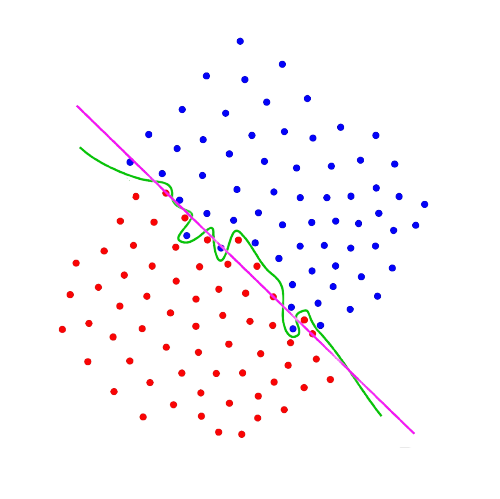
\includegraphics[width=8cm, height=5cm]{overfitting_clean.png}

\end{center}
\\ 

Podem observar que utilitzant el classificador de color verd obtenim una precisió del $100 \%$ a l'hora de classificar les dues categories en la mostra d'entrenament. Tot i aixo, és molt probable que si utilitzem el classificador amb noves dades independents a la mostra d'entrenament la precisió baixi de manera considerable. Aquest fet es podria haver evitat si en comptes de utilitzar el classificador verd haguéssim utilitzat el lila, el qual comet més errors en la mostra d'entrenament però segurament generalitza millor amb noves dades.

Les causes del sobreajustament en models de deep learning poden ser moltes, peró 



\section{Per què deep learning? Quines son les seves avantatges?}

Arribats a aquest punt ens podríem preguntar que fa tant especial aquests algoritmes. Quines son les característiques que els fan destacar per sobre de molts altres?

La raó principal és simple: Els algoritmes de deep learning ofereixen un millor rendiment en diversos problemes com ara la classificació d'imatges. Un exemple és el cas del problema ImageNet, el qual consistia en classificar imatges de gran resolució entre 1000 categories diferents entrenant els algoritmes amb una base de dades de 1.4 milions d'imatges. Fins al 2011 s'havien aconseguit precisions del $74.3\%$ amb algoritmes convencionals. No va ser fins un any més tard, el 2012 quan la implantació d'algoritmes de deep learning va prendre el lideratge en la competició assolint una precisió del $83.6\%$. Des de llavors aquesta precisió va anar millorant any rere any fins que al 2015 es va assolir una precisió del $96.4\%$ i es va considerar el problema ImageNet completament resolt. Des de llavors les xarxes neuronals han dominat el paradigma del reconeixement d'imatges (\textit{computer vision en anglès}) i també han assolit grans resultats en tasques com ara processament de llenguatge natural on en ambdós camps han substituït completament altres algoritmes d'aprenentatge automàtic com ara les màquines de suport vectorial (SVMs) o els arbres de decisió, algoritmes dels que parlarem més endavant en aquest projecte.

Com ja hem dit els algoritmes de deep learning ofereixen molt bons resultats en un gran ventall de problemes i aquesta és una de les raons per les quals s'han fet tant populars, però no és l'única. 

\subsection{Deep learning i feature engineering}

Un dels passos més importants en tot procés de machine learning és el feature engineering (enginyeria de característiques per la seva traducció literal). Aquest pas consisteix en seleccionar, manipular i transformar les dades originals que encara no han estat pre processades amb l'objectiu de millorar el rendiment dels nostres models i aixi obtindre millors resultats. Normalment aquests processos acostumen a ser llargs i tediosos però al mateix temps indispensables a l'hora de entrenar els nostres algoritmes.

En canvi, en el context del deep learning, es pot començar a partir de les dades sense pre-processar i les noves variables s'aniran creant a mida que la xarxa vagi aprenent. Aquest fet simplifica significativament tots els processos que tradicionalment és requerien a l'hora de treballar amb models, substituint diversos passos de processament per un únic model de deep learning que s'encarregara de tal labor.


\section{Un model alternatiu d'aprenentatge automàtic: Arbres de decisió i Random Forest}

Degut a la falta d'estabilitat en els nostres resultats amb xarxes neuronals provocats per diverses qüestions que ja hem exposat proposem un model alternatiu amb l'esperança de comparar els resultats amb els ja obtinguts prèviament i aixi satisfer l'objectiu principal del projecte: Utilitzar un model IA per optimitzar el funcionament de la UCI.

Hem triat els arbres de decisió com a model alternatiu per la seva senzillesa i bons resultats en conjunts de dades amb dimensions i estructura com el que tenim entre mans. En concret, prendrem una variant d'aquests arbres que combina els resultats de diferents models per tal d'evitar el sobreajustament, l'anomenat Random Forest. Peró no avancem els esdeveniments, parlem primer de que són els arbres de decisió i de com funcionen.

\subsection{Arbres de decisió}

Els arbres de decisió son models d'aprenentatge automàtic que no pertanyen al subconjunt de l'aprenentatge profund. Són fàcils d'interpretar i d'utilitzar però no són competitius amb els models de deep learning quan tractem amb quantitats enormes de dades. En casos amb conjunts de dades més reduïts com el nostre, poden ser de gran utilitat.

Els arbres es poden dividir en dues categories segons l'objectiu del problema a resoldre:
\begin{itemize}
    \item \textbf{Arbres de classificació:} 
    La variable que volem predir és categòrica i el model ens retornarà un conjunt de probabilitats per cada una de les categories possibles per cada un dels inputs. Per norma general assignarem la categoria amb la probabilitat més alta al input, però podem modificar el marge de decisió per tal d'obtenir resultats més satisfactoris.
    
    \item \textbf{Arbres de regressió:} 
    En aquest cas la variable a predir és continua i l'objectiu és predir el seu valor, com per exemple predir el preu del metre quadrat dels pisos en diferents zones d'una ciutat.
\end{itemize}

En el nostre cas com que el nostre objectiu és predir si un pacient tindrà o no complicacions ens centrarem en els arbres de classificació. En essència el que fa un arbre de decisió és dividir l'espai predictor en $K$ nodes que anomenarem fulles i cada node es caracteritza per una sèrie de normes. La predicció que retornarà el model per un input concret que compleixi totes les normes d'un node serà la moda d'aquest en la mostra d'entrenament. Aquests models comencen des de dalt dividint l'espai de les observacions en dos de forma binaria utilitzant un dels predictors. Una vegada tenim l'espai dividit en dos fem el mateix per cada un dels nous nodes utilitzant un altre predictor i així successivament fins que arribem als nodes inferiors o fulles utilitzant un criteri de parada. El següent esquema il·lustra molt bé com podriem procedir amb les nostres deades i predictors:

\includegraphics[scale=1]{}






https://tanthiamhuat.files.wordpress.com/2018/03/deeplearningwithpython.pdf

582x475

\section{Bibliografia}
Aprendizaje automático 1  Juan R González  2021-11-22  Grau d'estadística UAB

Deep learning with Python - François Chollet  editorial Manning

What is feature engineering: https://towardsdatascience.com/what-is-feature-engineering-importance-tools-and-techniques-for-machine-learning-2080b0269f10

Feature engineering is still necessary for deep learning: https://medium.com/inside-machine-learning/feature-engineering-for-deep-learning-2b1fc7605ace

Optimizers:
https://ruder.io/optimizing-gradient-descent/index.html#rmsprop

\section{Imatges}

https://towardsdatascience.com/dont-overfit-ii-how-to-avoid-overfitting-in-your-machine-learning-and-deep-learning-models-2ff903f4b36a

\end{document}